\documentclass[a4paper,12pt,oneside,onecolum,final,openany]{report} 

%---- Allgemeine Layout Einstellungen ------------------------------------------

% Für Kopf und Fußzeilen, siehe auch KOMA-Skript Doku
\usepackage[komastyle]{scrpage2}
\pagestyle{plain}
\setheadsepline{0.5pt}[\color{black}]
\automark[section]{chapter}


%Einstellungen für Figuren- und Tabellenbeschriftungen
\usepackage[utf8x]{inputenc} 
\usepackage[T1]{fontenc} 
\usepackage[ngerman]{babel} 
\usepackage{amsfonts} 
\usepackage{amsmath} 
\usepackage{tabularx}
\usepackage{float}

%---- Weitere Pakete -----------------------------------------------------------
% Die Pakete sind alle in der TeX Live Distribution enthalten. Wichtige Adressen
% www.ctan.org, www.dante.de

% Sprachunterstützung
\usepackage[ngerman]{babel}

% Benutzung von Umlauten direkt im Text
% entweder "latin1" oder "utf8"
%\usepackage[utf8]{inputenc}


% Pakete mit Mathesymbolen und zur Beseitigung von Schwächen der Mathe-Umgebung
%\usepackage{latexsym,exscale,stmaryrd,amssymb,amsmath}


\usepackage[nointegrals]{wasysym}
\usepackage{eurosym}

% Anderes Literaturverzeichnisformat
%\usepackage[square,sort&compress]{natbib}
\usepackage{hyperref}
% Für Farbe
\usepackage{color}
\usepackage{graphicx}
\usepackage{wrapfig}
\usepackage{subfigure}

% Caption neben Abbildung
\usepackage{sidecap}


% Befehl für "Entspricht"-Zeichen
\newcommand{\corresponds}{\ensuremath{\mathrel{\widehat{=}}}}
% Befehl für Errorfunction
\newcommand{\erf}[1]{\text{ erf}\ensuremath{\left( #1 \right)}}


%Fußnoten zwingend auf diese Seite setzen
\interfootnotelinepenalty=1000

%Für chemische Formeln (von www.dante.de)
%% Anpassung an LaTeX(2e) von Bernd Raichle
\makeatletter
\DeclareRobustCommand{\chemical}[1]{%
  {\(\m@th
   \edef\resetfontdimens{\noexpand\)%
       \fontdimen16\textfont2=\the\fontdimen16\textfont2
       \fontdimen17\textfont2=\the\fontdimen17\textfont2\relax}%
   \fontdimen16\textfont2=2.7pt \fontdimen17\textfont2=2.7pt
   \mathrm{#1}%
   \resetfontdimens}}
\makeatother
\usepackage{textcomp}
\usepackage{upgreek}
%\begin{document}
%$\upmu$
%\end{document}
%Honecker-Kasten mit $$\shadowbox{$xxxx$}$$
\usepackage{fancybox}

%SI-Package
\usepackage{siunitx}

%keine Einrückung, wenn Latex doppelte Leerzeile
\parindent0pt

%Bibliography \bibliography{literatur} und \cite{gerthsen}
%\usepackage{cite}
\usepackage{babelbib}
\selectbiblanguage{ngerman}

\usepackage{siunitx}
%\begin{document}
 % \SI{1.55}{\micro\metre}
\sisetup{math-micro=\text{µ},text-micro=µ}
\usepackage{amsmath}
\usepackage[verbose]{placeins}
\usepackage{setspace}
\usepackage{threeparttable}
\usepackage[verbose]{placeins}


\begin{document}

\begin{titlepage}
\centering
\textsc{\Large Physikalisch- Chemisches Grundpraktikum\\[1.5ex] Universität Göttingen}

\vspace*{0.5cm}

\rule{\textwidth}{1pt}\\[0.5cm]
{\huge \bfseries
  Versuch 3: \\[1.5ex]
  Differential Scanning Calorimeter}\\[0.5cm]
\rule{\textwidth}{1pt}

\vspace*{0.5cm}


\begin{Large}
\begin{tabular}{ll}
Durchführende: &  Isaac Maksso, Julia Stachowiak\\
Assistent: & Jannik Walter \\
 Versuchsdatum: & 17.11.2016\\
 Datum der ersten Abgabe: & 24.11.2016\\
\end{tabular}
\end{Large}

\vspace*{0.5cm}


\begin{table}[h]
\centering
\caption{Werte des Joule-Thomson-Koeffizienten für $\text{N}_2$.}
\begin{scriptsize}
\begin{tabular}{c|c|c|c} 
Temperatur/~°C&$ \mu_{\text{N$_{2}$,exp.}}$/~$\frac{\text{K}}{\text{bar}}$&$ \mu_{\text{N$_{2}$,th.}}$/~$\frac{\text{K}}{\text{bar}}$&$ \mu_{\text{N$_{2}$,Lit.}}$/~$\frac{\text{K}}{\text{bar}}$\\
\hline
0,1 & 0,181 $\pm$ 0,02& 0,252 &0,26$^1$\\
\hline
22,7 & 0,175 $\pm$ 0,02& 0,220&0,25$^2$\\
\hline
50,8& 0,120 $\pm$ 0,01& 0,173&0,19$^1$\\
\end{tabular}
\end{scriptsize}
\end{table}
\noindent
\FloatBarrier

\begin{table}[h]
\centering
\caption{Werte des Joule-Thomson-Koeffizienten für $\text{CO}_2$.}
\begin{scriptsize}
\begin{tabular}{c|c|c|c} 
Temperatur/~°C&$ \mu_{\text{CO$_{2}$,exp.}}$/~$\frac{\text{K}}{\text{bar}}$&$ \mu_{\text{CO$_{2}$,th.}}$/~$\frac{\text{K}}{\text{bar}}$&$ \mu_{\text{CO$_{2}$,Lit.}}$/~$\frac{\text{K}}{\text{bar}}$\\
\hline
0,1 & 1,20 $\pm$ 0,04& 1,21&1,31$^1$\\
\hline
22,8 & 1,01 $\pm$ 0,06& 1,05&1,12$^2$\\
\hline
50,8& 0,710 $\pm$ 0,05& 0,878&0,91$^1$\\
\end{tabular}
\end{scriptsize}
\end{table}
\noindent
\FloatBarrier

\vspace{1.3cm} 
\end{titlepage}


\tableofcontents %=Inhaltsverzeichnis
\newpage

\section{Einleitung}
Drei verschiedenen Stoffe (Indium, Polymethylmethacrylat "PMMA", Cyclohexan) sollen über ihren Phasenübergang betrachtet werden und die zugehörige Temperatur, Übergangsenthalpie und -entropie sowie die Wärmekapazitäten ermittelt werden.\\
Zunächst muss dabei die Ordnung des Phasenüberganges betrachtet werden. Bei Indium und Cyclohexan findet ein Phasenübergang erster Ordnung statt.Dabei gibt es eine definierte Temperatur bei der die Wärmekapazität unendlich ist, da jede zugeführte Energie in den Phasenübergang gesteckt wird. Während des Phasenüberganges befinden sich demnach zwei Phasen im Gleichgewicht.\\
PMMA ist ein Polymer, bei dem ein Glasübergang stattfindet, dh. ein Phasenübergang 2. Ordnung. Dabei ändert sich die Entropie kontinuierlich über eine Temperaturspanne hinweg. Von einem amorphen Festkörper findet der Übergang zu einer gummiartigen Masse statt.\\ 
Nach Ehrenfest hat der Phasenübergang die $n$-te Ordnung, wenn die $n$-te Ableitung von $G$ nach $T$, also z.B. bei der ersten Ableitung die Entropie sich nicht stetig, sondern unstetig ändert. Siehe dafür Gleichung (\ref{Ehrenfest1}) für einen Phasenübergang 1. bzw. (\ref{Ehrenfest2}) für einen Übergang 2. Ordnung.\\ 




\begin{equation} \label{Ehrenfest1}
\left(\frac{\partial G}{\partial T}\right)_p = -S
\end{equation}  
  
\begin{equation} \label{Ehrenfest2}
\left(\frac{\partial^2 G}{\partial T^2}\right)_p = -\frac{\partial S}{\partial T}= - \frac{c_p}{T}
\end{equation}  


Die molare Wärmekapazität bei konstantem Druck ist definiert als Temperaturänderung pro Wärmemenge. Durch den konstanten Druck gilt für $dH$ Gleichung(\ref{dH}). 

\begin{equation} \label{dH}
dH_p= TdS +Vdp =TdS
\end{equation}

Isobare Prozesse haben den Vorteil dass der letzte Term des totalen Differentials für $H$ wegfällt und die Entropieänderung leicht aus $dH$ berechnet werden kann (Gleichung \ref{EntropieEnthalpie}).\\


\begin{equation} \label{EntropieEnthalpie}
\left(\frac{dH}{T}\right)_p = dS
\end{equation}


\section{Experimentelles}
\subsection{Experimenteller Aufbau}
\begin{figure}[h]
\centering
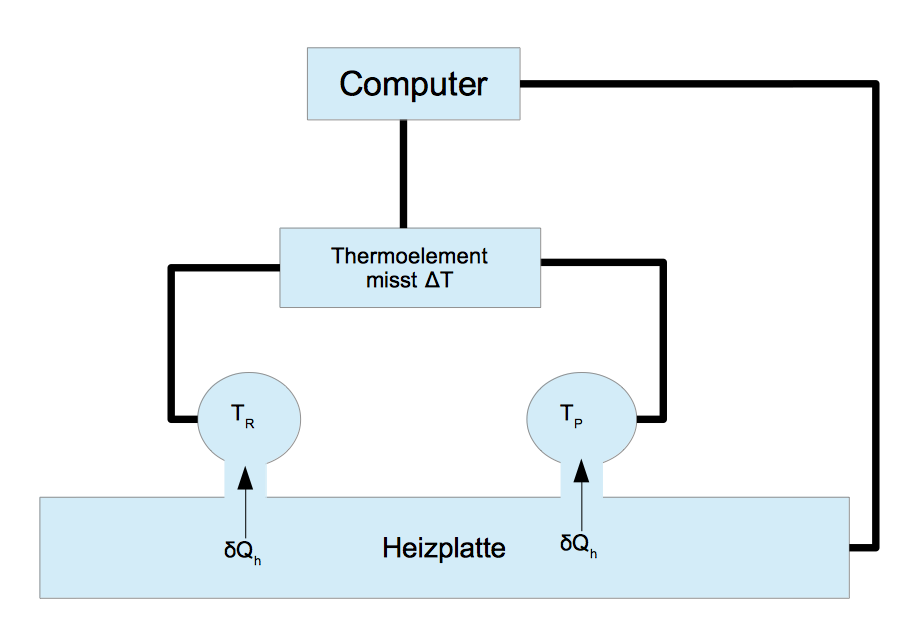
\includegraphics[width=13.5cm]{VB_SN.png}
\caption{Der Versuchsaufbau.}
\end{figure} 
\FloatBarrier
\subsection{Durchführung}
Das Dynamische Differenzkaloriemeter (DSC) wird hochgefahren. Dazu wird die Apparatur durch den Anschluss „Purge” \;mit einem Stickstoffstrom von ca. 50\;ml/min gespühlt. Der Druck wurde mittels einer Schwebkugel auf einen Wert von 70 eingestellt. Durch den Stickstoffstrom wird Wasser, welches die Messung beeinflussen könnte, in der Atomsphäre und dessen Kondensation verhindert. Die Probe des Indiummetalls lag in einer „crimp cell” \;vorbereitet vor. Es wurde zuerst Indium gemessen. Als Referenz wurde ein leeres Aluminiumpfännchen genutzt. Während des Messdurchgangs des Indiums wurde die Probe des Polymethylmethacrylat (PMMA) vorbereitet. Es wurde 19,7\;mg PMMA in eine „sealed cell” \;eingewogen. Die „sealed cell” \;wurde dann mittels einer hydraulischen Presse die Zelle mit einem Aluminium-Plättchen gasdicht verschlossen. Nach Abschluss der Messung des Indiums wurde die PMMA-Probe gemessen. Als Referenz wurde ein leeres Pfännchen eingelegt. Während der Messung der PMMA-Probe wurde die Cyclohexan-Probe vorbereitet. Es wurde ca. 0,03\;ml des Cyclohexans mittels einer 1-ml-Spritze in eine leere „sealed celle” \;gefüllt. Die Zelle wurde wie die PMMA-Probe mit einem Alumium-Plättchen als Deckel und einer hydraulischen Presse gasdicht verschlossen. Da bei der Messbereich der Cyclohexan-Messung unterhalb der Raumtemperatur liegt, wurde die Apparatur zusätzlich mit flüssigen Stickstoff gespühlt. Die Messergebnisse wurde mit dem Program \textit{TA60} ausgewertet.  
\section{Auswertung}
\subsection{Arbeitsweise und Anwendungsfelder eines DSC}
Ein "Differential Scanning Calorimeter" (DSC) misst bei gleichmäßiger Wärmezufuhr zu zwei Stoffen die resultierende Temperaturdifferenz.
Differential Scanning Kalorimeter lassen sich in 2 verschiedene Arten unterteilen: Power Compensation DSC und Heat-Flux DSC (in diesem Versuch verwendet). Bei Ersterem befinden sich Probe und Referenz in zwei verschiedenen Öfen, die auf die gleiche Temperatur geheizt werden. Die dafür aufgebrachten Heizleistungen werden verglichen und daraus die Enthalpiedifferenz $\Delta H$ bzw. die Differenz der molaren Wärmekapazitäten $\Delta C_\mathrm{m}$ ermittelt.\\
Beim Heat-Flux DSC wird beiden Stoffen die gleiche Heizleitung zugeführt und die resultierende Temperaturdifferenz mittels Thermoelement gemessen.\\
Bei einer geringen Temperaturdifferenz kann $C_\mathrm{m}(T)$ als konstant angesehen werden und aus den Differenzen $\Delta Q$ 

\begin{equation}
dH = TdS = \delta Q + \delta W +pdV
\end{equation}
 
Die verrichtete Arbeit wird über die Volumenänderung beschrieben, sodass letztendlich $\delta H = \delta Q$ gilt. So kann die Wärmekapazität nach Gleichung (\ref{cp}) beschrieben werden.\\

\begin{equation} \label{cp}
C_{\mathrm{m},p} =\frac{1}{n} \left(\frac{\delta Q}{\partial T}\right)_p =\frac{1}{n} \left(\frac{\delta H}{\partial T}\right)_p = \frac{1}{n} \left(\frac{\partial S}{\partial T}\right)_p= \frac{1}{n} \left(\frac{\partial^2 G}{\partial T^2}\right)_p
\end{equation}

Der letzte Schritt ist möglich da:\\

\begin{equation}
dG =-SdT -pdV
\end{equation}

\begin{equation}
\frac{dG}{dT}= -S
\end{equation}

Analog gilt für $\Delta C_{\mathrm{m},p}$.\\

\begin{equation}
\Delta C_{\mathrm{m},p} = \frac{1}{n} \left(\frac{\partial^2 \Delta G}{\partial T^2}\right)_p
\end{equation}



\section{Auswertung}
\subsection{Arbeitsweise und Anwendungsfelder eines DSC}
Ein "Differential Scanning Calorimeter" (DSC) misst bei gleichmäßiger Wärmezufuhr zu zwei Stoffen die resultierende Temperaturdifferenz.
Differential Scanning Kalorimeter lassen sich in 2 verschiedene Arten unterteilen: Power Compensation DSC und Heat-Flux DSC (in diesem Versuch verwendet). Bei Ersterem befinden sich Probe und Referenz in zwei verschiedenen Öfen, die auf die gleiche Temperatur geheizt werden. Die dafür aufgebrachten Heizleistungen werden verglichen und daraus die Enthalpiedifferenz $\Delta H$ bzw. die Änderung der molaren WÄrmekapazität $\Delta C_\mathrm{m}$ ermittelt.
Beim Heat-Flux DSC wird beiden Stoffen die gleiche Heizleitung $\Delta Q_\mathrm{h}$ zugeführt und die resultierende Temperaturdifferenz mittels Thermoelement gemessen.
Bei einer geringen Temperaturdifferenz kann $C_\mathrm{m}(T)$ als konstant angesehen werden und aus den Differenzen $\Delta Q$ und $\Delta T$ errechnet werden (Gleichung \ref{cp}).\\

DSC findet vor allem in der Polymerchemie Anwendung. Über durch die Bestimmung der Glasumwandlungstemperatur kann der Temperaturereich ermittelt werden, in dem das Material bearbeitet werden muss. Grundsätzlich kann Glas aus sehr verschiedenen Stoffen hergestellt werden, weist jedoch auch verschiedene Stabilitäten auf. Gleiches gilt für Kunststoffe. 
Sind $\Delta S$, $\Delta H$, $T_\mathrm{tr}$ und $c_p$ bekannt, so können Reaktionsgeschwindigkeitsgesetze aufgestellt und die benötigten Energien errechnet werden.\\ 
Ferner können auch Kunststoffe bestimmt werden.
Stoffe mit geordnetem Kristallgitter neigen eher zu einem Phasenübergang erster Ordnung; der "Peak" der DSC- Kurve ist dann relativ schmal. Bei unreinen Gittern ist der Phasenübergang  kontinuierlicher. So können mittels DSC auch Reinheits- und Kristallisationsgrad ermittelt werden.\\


\subsection{Rechnung}

Die Werte wurden aus dem Graphen nach Gleichung (\ref{cp}) von der Auswertungssoftware "TA60" berechnet. 
$\Delta S$ ergibt sich aus Gleichung (\ref{S}). Cyclohexan wurde mit steigender und abfallender Temperatur gemessen. Die tabellierten Werte sind die je die Mittelwerte der zugehörigen Kurve. Zur Berechnung wurden die Beträge der Werte der 2. Messung verwendet. Das Vorzeichen bezieht sich somit auf die 1. Messung.\\
Bei PMMA sind zwei Peaks zu sehen, obwohl nur einer zu erwarten war. Wahrscheinlich ist der zweite Peak durch einen Fehler aufgetreten, sodass in der Auswertung nur der erste und größere Peak berücksichtigt wurde. Da es sich bei PMMA um einen Phasenübergang 2. Ordnung handelt, kann nur der entsprechende Temperaturbereich ermittelt werden und nicht  \\

\begin{equation}\label{S}
\left(\frac{\Delta G}{T}\right)_p = \Delta S
\end{equation}


\begin{table} [h!]
\caption{Messwerte}
\begin{tabular}{c|c|c|c|c|c}
 & Stoffmenge $n$  & $T_\mathrm{tr}$  & $\Delta H$  & $C_{\mathrm{m},p} $ & $\Delta S$ \\ 
& [mol] & [K] & [J] & $[\mathrm{J} \cdot \mathrm{mol}^{-1}]$& [J $\cdot$ K$^{-^1}$] \\
\hline 
Indium & $232 \cdot 10^1$ & 432 & -0,57 & -322 $\cdot 10^1$ & -0,00132 \\ 
\hline 
PMMA 1.Peak & $1152 \cdot 10^2$ & 360,22 -397,43 & - & - & - \\ 
\hline 
Cyclohexan 1.Übergang & 279 & 5,70 & 0,475 & 1711 & 0,083 \\ 
Cyclohexan 2.Übergang & 279 & 187,4& 1,14 & 4111 & 0,00608 \\
\end{tabular}
\end{table}
\FloatBarrier










\section{Fehlerdiskussion}
$\Delta T$ muss sehr gering sein -> sonst ist Cm nicht konstant und auswertung falsch

2 Peaks bei PMMA

\section{Literaturverzeichnis}
1\quad Eckhold, Götz: \emph{Praktikum I zur Physikalischen Chemie}, Institut für Physikalische Chemie, Uni Göttingen, \textbf{2014}.

\vspace{0,5 cm}

2 \quad Eckhold, Götz: \emph{Statistische Thermodynamik}, Institut für Physikalische Chemie, Uni Göttingen, \textbf{2012}.

\vspace{0,5cm}

3 \quad Eckhold, Götz: \emph{Chemisches Gleichgewicht}, Institut für Physikalische Chemie, Uni Göttingen, \textbf{2015}.\\

\vspace{0,5cm}

4 \quad Atkins, P.W.: \emph{Physikalische Chemie}, Wiley-VCH, Weinheim, \textbf{2006}.\\

\vspace{0,5cm}

5 \quad Zemansky: \emph{Heat and Thermodynamics},Mc Graw-Hill, New York, \textbf{1990}.\\

\end{document}
